% So potentially the first chapter will be background on audio synthesizers
\chapter{Background}
\label{chapter:background}
- Research in this field is inherently interdisciplinary background covers many different areas including HCI, DSP, Machine learning
- What is the main goal? Reiterate here perhaps: "We want to develop a method for improving the user interface for synthesizer users" -- 
- In the field of HCI the study of creativity support tools is related to this:

\graphicspath{{./}{./figures/}{./figures/background/}}

\section{Audio Synthesizers}
In the context of audio, a synthesizer refers to a device that generates sound or music. Martin Russ provides a thorough overview of audio synthesis in his textbook, Sound Synthesis and Sampling \cite{russ2012sound}. Russ introduces the synthesizer as any device that gerates sound,  even the human voice can be thought of as a synthesizer, however, sound synthesizers have become more broadly accepted as an electronic device that produces synthetic sounds. A synthesizer may do this through the playback and recombination of pre-existing audio material or through the generation of raw audio waveforms. There are numerous types of synthesis techniques that are capable of producing a huge variety of different sounds. Broadly speaking, these sounds can be categorized into two different classes: `imitative` or `synthetic`. Imitative sounds attempt to emulate a sound that exists in the natural world such as a physical musical instrument or a sound effect such as an explosion. Electric pianos are examples of imitative synthesizers. Synthetic sounds are those that have no relation to a sound in the physical world. The distinction between imitative and synthetic sounds is blurry and most sounds fall somewhere in the middle. For example, synth-brass sounds, which were a staple of synths such as Roland's popular Jupiter-8, are sounds that are based on an imitation of a brass sound but extend into the synthetic realm. 

% This is maybe a bit more like introduction material?
Synthesizers have become ubiquitous in audio production and entire genres of music have been developed around their use. Bebe and Louis Barron produced the first electronic film score for the movie "Forbidden Planet" in 1955 using synthetic sounds. Since then the use of synthesizers for movies and video games has also become common-place.


\subsection{Evolution of Synthesizers}
A brief history of synthesizers is provided here for historical context to the development and use of synthesizers. The full history of the topic is beyond the scope of this thesis and the interested reader is referred to some great textbooks that cover audio synthesizers and their history \cite{roads1980interview, mcguire2015musical, jenkins2019analog, russ2012sound}, which were used in the writing of this chapter.
\subsubsection{Analog}
Until the late 1950s all synthesizers were analog. All analog synthesizers are defined by their use of continuous-time signals, as opposed to digital systems which operate in discrete chunks of information, or discrete-time signals. Early analog synthesizers can be broken down into two broad categories: (1) sounds that are generated directly by electric circuits by oscillating vaccuum tubes, or (2) rotating or vibrating physical systems that are controlled by electronic sources \cite{roads1996computer}. The first, as well as the largest sound synthesizer ever built was developed in the early 1900s by Thaddeus Cahill. On September 26, 1906, an audience of 900 individuals came to view the massive electronic instrument called the Telharmonium that was capable of producing pure sinusoidal waves in at frequencies in integer ratios. Other early synthesizers include the Theremin, built by Leon Theremin in 1920, which produced a pure tone with a varying pitch and amplitude that was controlled by a performer moving their arms in relation to two antennas. The sound produced by the theremin has an eery feel to it, well-suited for sci-fi film scores. Versions of the theremin have been used in popular music by musicians including The Beach Boys, Led Zeppelin, and The Rolling Stones (citations? check out wikpedia).  The Ondes Martenot, developed in 1928 by Maurice Martenot and Ondes, had a similar sound to the theremin and also was one of the first synthesizers to include a piano-like keyboard interface.

In the 1960s two companies emerged on opposite sides of America and released synthesizers that have shaped the landscape of audio synthesis. Around 1964 Don Buchla, who lived in the San Francisco area, released the the Buchla 100 Series Modular Electronic Music System and Robert Moog, who lived in the New York area, released the R.A. Moog Modular System \cite{mcguire2015musical}. Both synthesizers were modular systems that had individual processing units called \textit{modules} that could be interconnected using patch cables, connecting together synthesizer modules is known as creating a "synth patch", or simply a "patch". Both systems also include Voltage-Controlled Oscillators (VCOs) which create electronic waveforms at stable musical pitches, and the pitch can be controlled via an input signal. The Moog Modular System also featured a Voltage Controlled Filter (VCF) that was an early version of Moog's famous ladder filter design that would resonate at a controllable center frequency, creating some of the most iconic synthesizer sounds that are still used today.

There were some important philosophical differences between Moog and Buchla Synthesizers that have lead to two different schools of thought: East Coast and West Coast synthesis. The development of the Buchla synthesizer by Don Buchla was guided by Morton Subotnick and other experimental composers working out the San Francisco Tape Music Center. Subotnick explicitly requested that the synthesizer was not controlled by a traditional keyboard interface as he was worried that it would trap him into created tonal music. Instead, Buchla synthesizers are controlled using a set of touch plates and sequencers. At the same time on East coast Robert Moog was developing the Moog Modular and building a traditional keyboard interface to control the pitch of his VCOs. This feature, which allowed the Moog Modular Systems to be integrated more easily with Western music, was one of the reasons that Moog synthesizers became much more popular and commercially successful compared to Buchla. 

Another reason that Moog synthesizers were launched into the public eye is because of their use in recorded music. In 1968 Wendy Carlos used a Moog Modular synthesizer to orchestrate, perform, and record a selection of Johann Sebastian Bach pieces. The collection of music, called \textit{Switched On Bach}, went on to become the best selling classical recording of all time. Other musicians had created recreations of classical music pieces on synthesizers, but none had reached the same level as \textit{Switch On Bach}. Jenkins \cite{jenkins2019analog} credits the nature of the counterpoint in Bach's pieces as being particularly well suited to synthesizers, as well as Carlos' ability to design sounds that brought that performance alive, to the success of the release. Building on this success Carlos went on to score synthesized soundtracks for movies including Stanley Kubrick's \textit{A Clockwork Orange}. Another exceptional example of classical music recreated using Moog synthesizers worth mentioning is Japanese composer Isao Tomita's \textit{Snowflakes Are Dancing}, which was released in 1974. The use of synthesizers in music and film extends into almost all genres of music and was the cornerstone in the development of new genres including techno and other electronic music genres. [Also note something about the historical context and other synthesizer manufacturers] -> Mark Jenkins provides an excellent overview of the use of synthesizers in various genres of music over the years in his book \textit{Analog Synthesizers: Understanding, Performing, Buying} \cite{jenkins2019analog}.

\subsubsection{Digital}
The first experiments with digit synthesis were conducted by Max Mathews on an IBM 704 computer in 1957 \cite{roads1980interview}. These experiments consisted of programming and synthesizing melodies using triangle waves, Mathew's program was able to accept the note pitch, amplitude, and duration. The Music III program was developed by Mathew's in 1960 and introduced an important concept called the \textit{unit generator}, which defined basic components of a synthesizer in programmatic units that a user was able to link together to create a full synthesizer architecture. Mathew's describes these concepts as being developed in parallel, but separately, to similar synthesis concepts (e.g. modular synthesizers) being developed in the analog world. He described this as "an advantage because a musician who knew who to patch together Moog synthesizer units would have a pretty good idea how to put together unit generators in the computer."

In 1973 John Chowning, a researcher at Stanford, released a landmark audio synthesis paper entitled on Frequency Modulation (FM) synthesis \cite{chowning1973synthesis}. The patent for FM synthesis was licensed to Yamaha who developed the Yamaha DX7 synthesizer using the technology, which was released in 1983 and became one of the best selling synthesizers of all time. One of the major benefits of FM synthesis is that it is able to produce complex audio waveforms at low computational cost. Additionally, the Yamaha DX7 was a fully polyphonic synthesizer, meaning that it was capable of producing multiple tones simultaneously (i.e. was able to play chords), whereas most analog synthesizers that were within the same time period were monophonic (only capable of playing one note at a time). The Yamaha DX7 was also incredibly difficult to program, although it came preloaded with a large selection of quality parameter settings, or presets, that allowed users to play the synth without have to learn how to program it.

As digital technology improved and computers became more powerful, new synthesis techniques such a sampling synthesis \cite{mcguire2015musical} and physical modelling \cite{jaffe1983extensions} emerged. Digital emulations of analog synthesizers, or virtual analog (VA) synthesis, also started to become popular in the 1990s. VA synthesizers attempt to express traditional analog synthesis methods in code as digital signal processing (DSP) algorithms. The development of more powerful computers also enabled recording workflows to be transferred into software and professional recording studios started to transition to digital with the release of Digidesign ProTools in the early 1990s. As software synthesis became more prevalent, many types of different software synthesizers emerged including VA software synthesis and a trend emerged of directly emulating analog equipment digitally, including the user interface. Skeumorphism describes computer user interfaces that attempt directly mimic their real-world counterpoint, and has become extremely common in audio software, including synthesizers; user interface researchers have begun to question whether or not these skeumorphic interfaces enhance usability of not \cite{lindh2018beyond}.

\subsubsection{Audio Plugins}
In 1996 Steinberg\footnote{\url{https://www.steinberg.net}} released the Virtual Studio Technology (VST) interface, which allowed third-party software including audio effects to be integrated into host applications including DAWs. Because VSTs integrate with host applications, they are also called audio plug-ins. The second version of VST was released in 1999 which added support for the Musical Instrument Digital Interface (MIDI) \cite{rothstein1992midi}, a communication protocol enabling musical hardware and software to exchange information and control signals. The addition of MIDI to the VST interface opened the doors for VSTi, VST instruments, including software synthesizers. Other audio plug-in architectures have been developed in addition to VSTs, and popular ones include Apple's Audio Units (AU) and Avid's Avid Audio eXtension (AAX). Audio plug-ins have allowed software developers a method to create unique audio effects and synthesizers, and an industry dedicated to their development has blossomed over the last few decades. At the time of writing there are over 500 different synthesizer plug-ins available for purchase or for free on the KVR\footnote{\url{https://www.kvraudio.com/plugins/softsynth-virtual-instruments}} database of audio products.

\subsection{Components of a Synthesizer}
Synthesizers can be viewed as comprising two major components: the synthesis engine, which is where sounds is generated, and a control interface which allows a user to control the synthesis engine \cite{russ2012sound}. Audio synthesis can be a complex process, so there is generally a high-level of abstraction between the synthesis engine and the control interface. The role of the control interface is to present a conceptual model of the synthesizer to a user, which allows the user to express their ideas and modify the synthesis engine. The parameters on the control interface are mapped to components within the synthesis engine, often in non-linear and complex ways. Figure \ref{fig:synth_abstraction} shows a diagram of the general components of a synthesizer and the control interface abstraction layer. The following sections provide more detail on each of the two major components of a synthesizer.

\begin{figure}[ht]
    \centering
    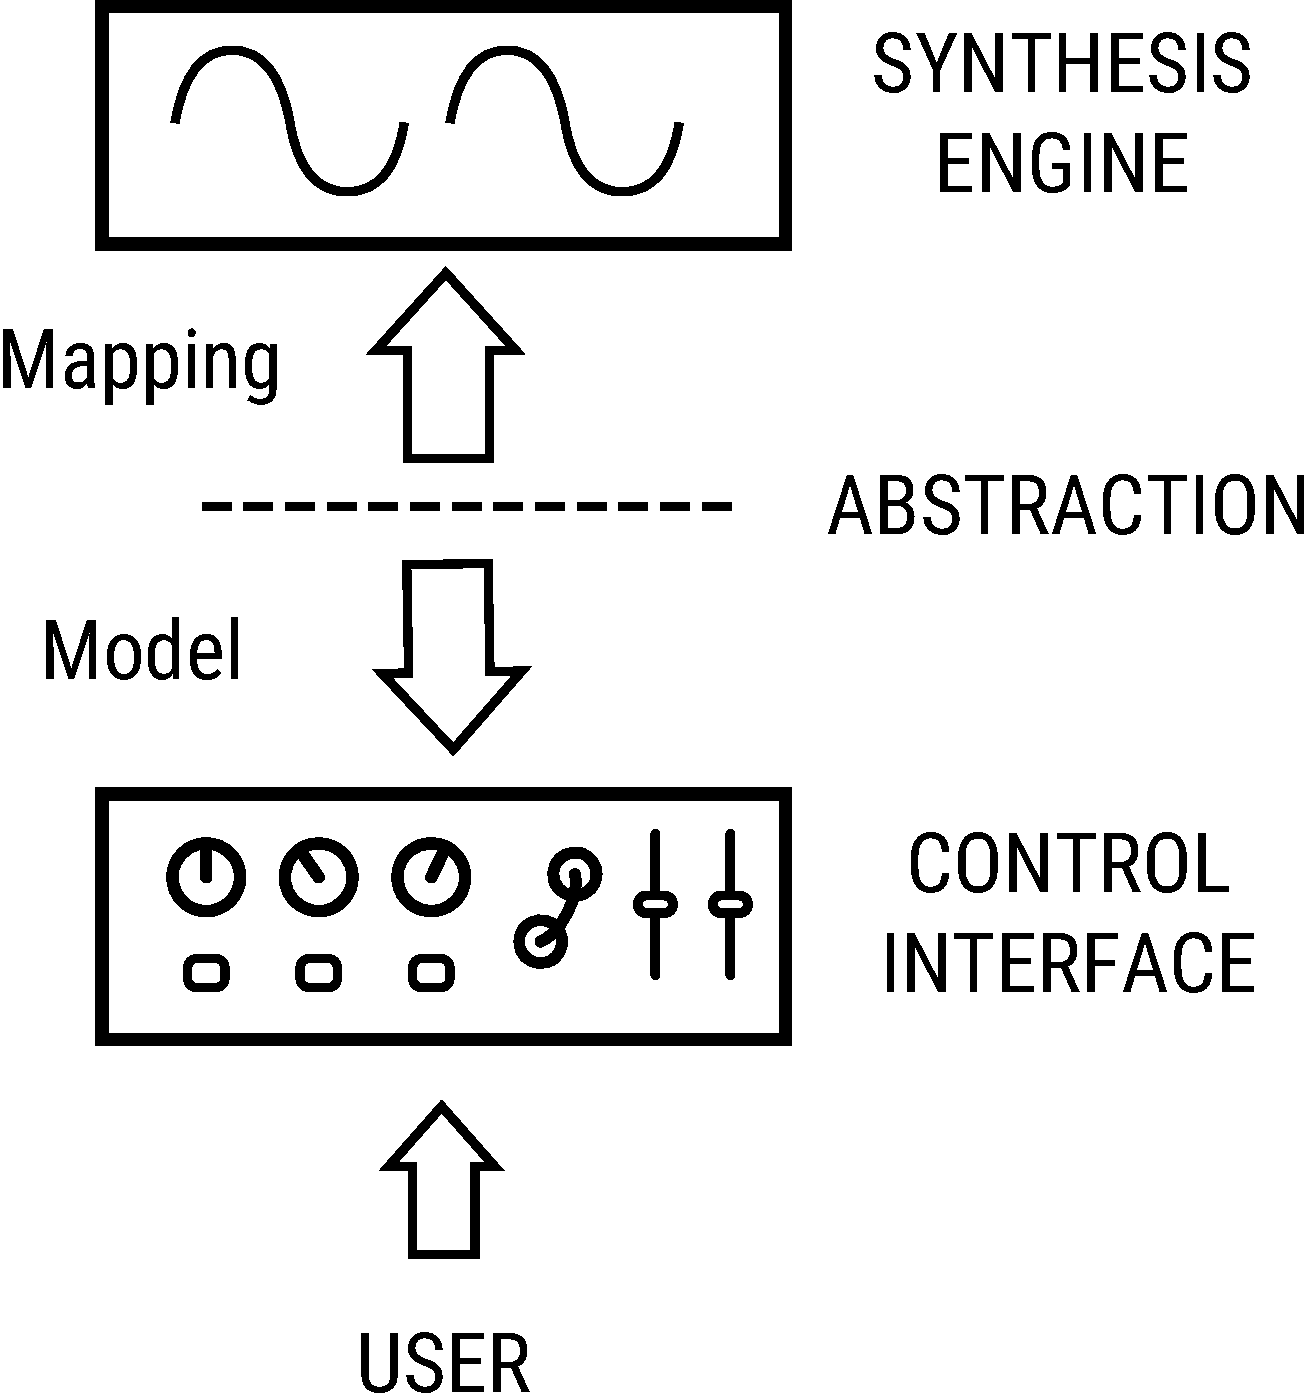
\includegraphics[width=0.4\textwidth]{figures/background/Synth Abstraction Model.pdf}
    \caption{Abstraction between the synthesis engine and control interface. A control interface on a synthesis is responsible for presenting a conceptual model of the underlying synthesis engine to a user. The parameters on the control interface are mapped back to the synthesis engine to modify audio generation.}
    \label{fig:synth_abstraction}
\end{figure}

\subsection{Synthesis Engine}
The synthesis engine is at the heart of sound generation in any synthesizer, whether it is an analog modular synth or a software audio plugin. There have been many different approaches to sound generation, and it is an active field with researchers and audio developers continuing to look for novel ways to create sounds. Sam McGuire and Nathan Van der Rest provide a good overview of some of the more popular synthesis methods in their book \textit{The Musical Art of Synthesis} \cite{mcguire2015musical}. These methods include: subtractive, sample-based, modulation (i.e. FM), additive, wavetable, granular, vector, and physically modelling. 

While the exact technique that each of these methods use may be different, there are some common components to synthesizers that exist in some form across different techniques. It is useful to take a modular perspective when thinking about different synthesizer components, similar to the \textit{unit generator} concept introduce by Max Mathews \cite{roads1980interview}, in which different components of a synthesizer are broken down into functional units (modules) that can be interconnected in various ways. We can generalize modules as all producing some output signal as well as having an optional input signal. Modules may also have some parameters that can be mapped to a control interface to enable user control. We can broadly categorize the signals that are output by modules as either audio signals or control signals. Audio signals are generated by the synthesizer and ultimately are output as a sound. Control signals are used to modulate the parameters of other modules within a synthesizer. In some synthesizers audio signals can also be treated as control signals and be used to modulate parameters of other parameters.

We can categorize modules into two different types based on the type of signal they output: 1) \textbf{audio modules}, generate or process audio signals, and 2), \textbf{control modules}, generate or process control signals. Jenkins provides an overview of some of the different synthesizer modules from the perspective of an analog synthesizer \cite{jenkins2019analog}. In analog synthesis audio signals are commonly generated by voltage-controlled oscillators (VCOs). In a VCO the frequency of the oscillator is controlled by the voltage of an input control signal. While voltages only exist in analog circuits, the concept has been extended into digital synthesizers as well, with the digital equivalent of a VCO sometimes being referred to as a digitally controlled oscillator (DCO). Other common audio modules are voltage-controlled filters (VCFs), voltage-controlled amplifiers (VCAs), and Noise Sources; filters accept audio signals as input and attenuate or boost specific frequencies, VCAs are essentially an automated volume knobs, and noise sources generate different types of noise such as white noise.

Exploring all of these methods in detail is beyond the scope of this thesis, however two methods are particularly relevant to the methods explored: subtractive synthesis and frequency modulation (FM) synthesis. 


\subsubsection{Subtractive Synthesis}
Subtractive synthesis was one of the earliest methods explored and is the sound of the famous Moog synthesizers. It has been used on thousands of records, and is still a popular method. The basic idea behind subtractive synthesis is that the starting point is a harmonically rich waveform, generated by an oscillator, which is then sent through a chain of filters and other audio effects that shape the timbre of the waveform over time. [Insert a simple block diagram of a subtractive synth]. There are several types of waveforms that are generally available on a oscillator in a subtractive synthesizer, these are shown in figure X [insert a diagram of some of the common waveforms and their harmonics]. Each waveform has a unique set of harmonics. Harmonics refer to frequencies that are present in the sound that occur at integer frequency ratios to the fundamental frequency of the sound, which is associated to the perceived pitch of that sound. Sine waves are the simplest waveforms and only contain energy at the fundamental frequency. Noise generators produce energy at all frequencies and contain no fundamental frequency and are therefore inharmonic.

Once a waveform has been generated it may be combined with other waveforms through a process called mixing. The average subtractive synthesizer has three oscillators \cite{russ2012sound} that are typically tuned to harmonically related frequencies. The next common stage in a subtractive synth signal path is an audio filter. As previously mentioned, one of the most famous synthesizer filters of all time is the Moog ladder filter \cite{moog1965voltage}, which is a resonant low pass/high-pass filter. Low pass filters allow low frequency sounds to pass through while attenuating frequencies above a certain threshold frequency, vice-versa for high-pass filters. The threshold frequency is usually controllable and can be modulated using other signals to create dynamic 'sweeping' sounds. After passing through the filter the signal passes through an amplitude gate, which acts as a volume knob that is controlled by an internal control signal envelope. The envelope 



\subsubsection{Frequency Modulation Synthesis}
FM synthesis was an another early method of synthesis that was developed during the origins of digital synthesis methods. FM synthesis engines are capable of produce a huge array of complex waveforms using a relatively simple stucture, which makes them powerful, however more conceptually challenging to understand compared to subtractive methods. The basic unit of an FM synthesizer is referred to as an operator, which generally contains a single simple sine wave oscillator and an amplitude gate controlled by an envelope generator. The simplest FM synthesizer consists of two operators that are connected together in way so that one of the operators controls the frequency of the second operator. The operator that does the modulating is referred to the \textit{modulator} and the operator that is modulated is referred to the \textit{carrier}. [Insert figure showing this arrangement.]

\subsubsection{Neural Synthesis}
One area of new development in audio synthesis is in methods that are leveraging advancements from the field of deep learning [deep learning cite], an area of audio synthesis that is explored in this thesis.  


- Pretty much just give a listing of techniques here. Potentially give a bit more of an overview of substractive vs. FM.
- Sound Synthesis and Sampling provides a thorough overview of both analog and digital synthesizers and the various methods. \cite{russ2012sound}

\subsection{Control Interface}
The control interface presents a conceptual model of the synthesizer to the user and maps this model to the underlying engine. A control interface has a set of parameters that can be altered to modify the nature of the sound being generated. A skilled sound designer is able to interact with the control interface and craft sounds to fit the needs of their creative project. This process is referred to as programming a synthesizer. A well-designed synthesizer control interfaces allow users to build up a conceptual model that allows them to easily interact with the synthesizer in a way that allows them to be expressive. 

% Not so sure about this section.
% The nature of the control interface is guided by the synthesis method being used by the engine. Synthesis methods like subtractive synthesis which involve a clear linear signal flow that starts with a complex waveform that is progressively shaped can lead to a more simple conceptual model. Moog synthesizers are examples of subtractive synthesizers that have clear control interface that maps to the synthesis engine. More complex synthesis methods such as Frequency Modulation (FM) synthesis are more challenging to create clear control maps for. Interestingly, the most commercially successful synthesizer, the Yamaha DX7, had a notoriously difficult control interface, although shipped with an extensive high-quality set of factory presets (pre-defined control interface parameter settings).

\subsection{Synthesizer Programming}
Both Carlos and Tomita excelled at patching synthesizer modules together and tuning the parameters of individual modules to create new sounds to orchestrate their performances. This process ... it's art! Blah blah blah. But also these folks are artists and virtuosos.

- Challenges with synthesizer programming UI design: \cite{seago2013new}. -- "Some, like subtractive synthesis, offer controllers which are broadly intuitive, in that changes to the parameter values produce a proportional and predictable change in the generated sound. Other methods, however, are less easily understood. FM synthesis, for example, is a synthesis method that may be viewed as essentially an exploration of a mathematical expression, but whose parameters have little to do with real-world sound production mechanisms, or with perceived attributes of sound." -- There are some other really good bits about navigating the timbre space and non-linearities.
- \cite{seago2004critical} Thus, under most current systems, the user is obliged to express directives for sound specification in system terminology, rather than in language derived from the user domain. Three types of synthesizer interfaces: parameter selection in a fixed architecture, architecture specification and configuration, and direct specification of physical characteristics of sound.
- Context on synthesizer programming \cite{jenkins2019analog}
- Russ describes the programming component intrinsically creative.
- When we talk about programming synthesizers we are referring to the task of selecting parameter settings for a synthesizer in order to achieve a desired sound
- Talk about the nature of this task. I think in that krekovic study there was something about this process? That this can be done in an exploratory way that ppl enjoy that process.
- Even so, it can still be quite a challenging task.

Programming audio synthesizers is challenging and requires a technical understanding of sound design to fully realize their expressive power. Traditional synthesizers can have over 100 parameters that affect audio generation in complex, non-linear ways. One of the most commercially successful audio synthesizers, the Yamaha DX7, was notoriously challenging to program. Allegedly nine out of ten DX7s coming into workshops for servicing still had their factory presets intact \cite{seago2004critical}.

Give an image of the complex synth UI.

% Bounce this out to another section I think. This could sit in creativity support potentially?
% \subsubsection{Neural Synthesis}
% In contrast to traditional synthesis, neural synthesizers generate audio using large-scale machine learning architectures with millions of parameters \cite{engel2017neural}. Differentiable digital signal processing \cite{engel2020ddsp} bridged the gap between traditional DSP synthesizers with the expressiveness of neural networks, exploring a harmonic model-based approach, using a more compact architecture with 100K parameters.
% One benefit of synthesized audio is that the underlying factors of variation ({\em i.e.}~the parameters) are known.

% % GANs for synthesis
% In this work, we use Generative Adversarial Networks (GANs) \cite{goodfellow2014generative} to generate new instrumental audio from a dataset of existing material. GANs have the potential to be used to generate new sounds on the fly. This would dramatically alleviate both the problem of having to pore through giant sound libraries, and the problem with having to only use one sample repeatedly. In addition, the explosion of new sounds which could potentially be produced by GANs would vastly reduce recording costs by designers of sound libraries.

% This research avenue is to a certain degree untapped: GANs have been successfully applied to the generation and manipulation of images, however, relatively little work has been focused on the audio domain. Research related to the specific work proposed here was presented by \cite{donahue2018adversarial}  and \cite{engel2018gansynth}.


\section{Synthesizer Programming}
Users generally have two options when trying to generate a desired sound on a synthesizer: they can build up the sound from scratch by adjusting parameters, or they can use a preset parameter setting designed by someone else. Many users also use presets as a starting point and manually adjust parameters to tune the sound \cite{krekovic2019insights}. Synthesizer programming refers to the process of manually adjusting parameters, whether starting from scratch or a preset. Programming a rich sound is considered an art \cite{russ2012sound}, and the quality of the sounds designed by Carlos and Tomita are one of the reasons their work achieved critical acclaim \cite{jenkins2019analog}. Specific techniques for programming synthesizers have lead to the production of sounds that define genres of music, especially electronic music, such as the "wobble bass" sound characteristic of dubstep. [What else can I add here to describe the importance of sound design? Is there anything else?]

\subsection{Challenges}
\subsubsection{Timbre}
In the previous section on synthesizer control interfaces, \S\ref{sec:control_interfaces}, three different dimensions of sound were introduced: pitch, loudness, and timbre. Pitch and loudness are uni-dimensional and have relatively simple mappings to parameters \cite{seago2004critical}. The remaining parameters on a synthesizer, which is the vast majority of them, are used to specify the timbre of the resulting sound. Musical timbre, unlike pitch and loudness, is multidimensional and challenging to understand \cite{krumhansl1989musical}. The ANSI definition of timbre is that it is the attribute of auditory sensation that allows it to be distinguished from other sounds at the same pitch and loudness \cite{american1973american}. This definition doesn't tell us very much about what timbre is, as opposed to what it is not. Risset and Wessel \cite{risset1999exploration} explore timbre in the context of audio synthesizers ... [what does this add?]

The artistry in synthesizer programming lies in the specification of parameters to create new musical timbre.

- Seago defines the procress of programming a synthesizer as selecting the timbre. \cite{seago2004critical}

- Synthesizer programming is essentially like trying to navigate the space of timbre.
- Risset and Wessel \cite{risset1999exploration} on timbre and synthesis.
- What can we say about timbre space? How can we define timbre? \cite{grey1977multidimensional}. Grey created a three-dimensional representation of timbre.
- \cite{bates2021interface} - looks at interfaces of modular synthesizers (maybe better in control interfaces?) 
- \cite{d2016interface} interface of software synthesizers and smart phones?

A skilled sound designer is able to interact with the control interface and craft sounds to fit the needs of their creative project. This process is referred to as programming a synthesizer. 

Both Carlos and Tomita excelled at patching synthesizer modules together and tuning the parameters of individual modules to create new sounds to orchestrate their performances. This process ... it's art! Blah blah blah. But also these folks are artists and virtuosos.

- Challenges identified in \cite{ethington1994seawave}: Timbre is most commonly specified by a large collection of numerical parameters peculiar to a particular synthesis technique."
- Challenges with synthesizer programming UI design: \cite{seago2013new}. -- "Some, like subtractive synthesis, offer controllers which are broadly intuitive, in that changes to the parameter values produce a proportional and predictable change in the generated sound. Other methods, however, are less easily understood. FM synthesis, for example, is a synthesis method that may be viewed as essentially an exploration of a mathematical expression, but whose parameters have little to do with real-world sound production mechanisms, or with perceived attributes of sound." -- There are some other really good bits about navigating the timbre space and non-linearities.
- \cite{seago2004critical} Thus, under most current systems, the user is obliged to express directives for sound specification in system terminology, rather than in language derived from the user domain. Three types of synthesizer interfaces: parameter selection in a fixed architecture, architecture specification and configuration, and direct specification of physical characteristics of sound.
- Context on synthesizer programming \cite{jenkins2019analog}
- Russ describes the programming component intrinsically creative.
- When we talk about programming synthesizers we are referring to the task of selecting parameter settings for a synthesizer in order to achieve a desired sound

- Talk about the nature of this task. I think in that krekovic study there was something about this process? That this can be done in an exploratory way that ppl enjoy that process. \cite{krekovic2019insights}
- 122 participants. 71\% had ten or more years of experience using synthesizers and only 2.7\% claimed they were novice users. Also, a majority of users had some formal training as musicians. So this study has quite a high representation of users who are experienced, as opposed to studying individuals who are novices. Musical training was only a weak indicator of experience using synthesizers. Most users most often create a synth patch from scratch or modify an existing one and only sometimes use presets with no modification. Interestingly there was no correlation with experience or music education. All users, regardless of experience or musical knowledge most often tweak the parameters of synthesizers.
- Four impediments to manually programming a synthesizer: 1) It can be time consuming, 2) it can distract them from focusing on music, 3) it can be difficult and non-intuitive to learn how to use a particular instrument, and 4) it rarely leads to desirable results. Participants agreed with the first three statements. Most participants disagreed with the fourth statement, but users with less experience were more likely to agree. Considering the average experience level of the group, these results highlight the challenges with synthesizer programming in the context of creating music.

- Even so, it can still be quite a challenging task.

% Potentially introduction material
Programming audio synthesizers is challenging and requires a technical understanding of sound design to fully realize their expressive power. Traditional synthesizers can have over 100 parameters that affect audio generation in complex, non-linear ways. One of the most commercially successful audio synthesizers, the Yamaha DX7, was notoriously challenging to program. Allegedly nine out of ten DX7s coming into workshops for servicing still had their factory presets intact \cite{seago2004critical}.

\subsection{Opportunities}
Krekovi\'{c} \cite{krekovic2019insights} participants were also asked to rate the perceived helpfulness of improvements to synthesizer  interfaces. Four different systems were proposed: 1) random presets are generated within a category, 2) a user provides a description of a the desired sound and a preset is generated for them, 3) a user provides an example sound and the system generates a presets to sound similar, and 4) more intuitive interactive user interface. Participants thought that proposed systems 3 and 4 would be helpful and systems 1 and 2 would be slightly helpful.

\section{Creativity Support}
The field of creativity support is focused on the development of tools to enable and enhance the creative output of an individual or group, both in novice and expert users. Creativity support tools (CSTs) \cite{shneiderman2007creativity} span a wide array of application domains including visual art, textiles, cooking, and music. A central question that CSTs ask is: 
\begin{quote}
    "How can designers of programming interfaces, interactive tools, and rich social environments enable more people to be more creative more often?"
\end{quote}
 Shneiderman \cite{shneiderman2007creativity} outlines a set of design principles for developing creativity support tools which include: support exploratory search, enable collaboration, provide rich history keeping, design with low thresholds, high ceilings, and wide walls. In subsequent related work, Davis \textit{et al.} focus on the role that CSTs play in supporting novices engaging in creative tasks and the relationship that the environment plays in creativity \cite{davis2013toward}. In their work, the authors identify two types of novice users: domain novices and tool novices. Domain novices are new to both the creative domain as well as using the creativity support tool. Tool novices have experience with the creative domain, but are novices at using a particular tool. To help evaluate and promote the development of creativity support tools for novices, they also propose a theory of creativity support based on cognitive theory.

These concepts provide an important platform for beginning to develop tools to support users of synthesizers. Both types of novices described by Davis \textit{et al.} are common and serve to benefit from the development of improved methods for interacting with them; domain novices are both new to sound design / music production as well as to using a specific synthesizer, whereas a tool novices would likely have experience with sound design / music production, but would be a novice with using a specific synthesizer. 

\subsection{Music Information Retrieval}
The field of music information retrieval (MIR) is a growing research area that was born out of the need to navigate increasingly large collections of digital music. Creative MIR is a subset of the field that is focused on applying the techniques from MIR towards creative applications including music production \cite{humphrey2013brief}.

- Conversations with music producers: \cite{andersen2016conversations}

- More directly related to music the fields of MIR (creative MIR) as well as intelligent music production. - automatic mixing ref, other topics (hit up some references and expand on this)

- Overview of approaches in intelligent music production \cite{moffat2019approaches}, automatic mixing \cite{de2017ten}.

- MIR audio querying: Automatic synthesizer programming can be viewed as a retrieval task as well as an optimization problem. Viewed as a retrieval task, the problem is similar to the MIR query tasks such as Query-by-example \cite{zloof1977query}, Query-by-vocal-imitation \cite{blancas2014sound}, and query-by-beat-boxing \cite{kapur2004query}. Query problems generally build up a model of the synthesis parameter space and then return a parameter setting based on a classification that attempts to match the input with the best parameter setting.
- Visualizing sounds: \cite{wessel1979timbre} (Potentially add the George citation on visualizing sounds).

- \cite{pardo2019learning} "Learning to build natural audio production interfaces" -> Rather than force nonintuitive interactions, or remove control altogether, we reframe the controls to work within the interaction paradigms identified by research done on how audio engineers and musicians communicate auditory concepts to each other: evaluative feedback, natural language, vocal imitation, and exploration
% This could potentially be its own section
\section{Audio Representations}
- how do we represent audio digitally?
- That tutorial by that ableton author was helpful -- maybe can link to that.
- Don't go into too much depth here.
- What is a perceptually relevant method for representing audio?
- Spectral features
- STFT

% Not totally sure how to incorporate these sections?
\subsection{Learned Audio Representations}
- Representation learning \cite{bengio2013representation}
- Introduce machine learning
- self-supervised learning
- Learned audio representations
- Give a brief plug for HEAR 2021 and the need for perceptual audio representations

% Unsure whether or not this is going to be its own chapter yet ...
\chapter{Automatic Synthesizer Programming}
\label{chapter:asp-background}
- The field of ASP has been an active area of research for 40+ years.
- What did the early work have to say about programming synthesizers? Why did the early work exist?
- This chapter provides background to the field of automatic synthesizer programming and 


\section{Automatic Synthesizer Programming}
Early ASP research emerged in the late 1970s with work that focused on the use of analytic methods to estimate the parameters for frequency modulation (FM) synthesis \cite{justice1979analytic}. That work was an example of synthesizer sound matching in which a system estimates synthesizer parameters to replicate a target sound. Since then a large volume of work on synthesizer sound matching has been published and has explored a variety of synthesis techniques and algorithmic methods.
- other early methods focuses on analytic methods for programming synthesizers \cite{beauchamp1982synthesis, payne1987microcomputer, delprat1990parameter}

- Research by Benjamin Hayes on the timbre space of synths -- looks super interesting.

Since the early 90s, researchers have leveraged advances in ML to develop a deeper understanding of the synthesizer parameter space and to build more intuitive methods for interaction \cite{horner1993machine}. Recently, deep learning has been used for programming synthesizers.  Esling {\em et al.}\ \cite{esling2020flow} trained an auto-encoder network to program the \href{https://u-he.com/products/diva/}{U-He Diva} using 11K synthesized sounds with known preset values. Yee-King {\em et al.} \cite{yee2018automatic} used a recurrent network to automatically find parameters for \href{https://asb2m10.github.io/dexed/}{Dexed}, an open-source software emulation of the DX7.

- In this section an overview of the field of automatic synthesizer programming is presented. Specific emphasis is placed on the HCI aspect of the problem and an overview of various user interaction methodologies is provided here.
- Inverse synthesis, a subset of automatic synthesizer programming and a focus of this thesis, is reviewed in more detail in the following section.
- This chapter concludes with a categorization of work in automatic synthesizer programming research that has been conducted over the last 30 years.

\subsection{User Interaction}
- This is really a user interface problem. Programming synthesizers is hard!
- What are some of the different approaches that have been taken by people?
- Interactive methods (IGAs)
- Semantic search
- That interesting paper on sketching sounds visually
- Pardo look at how we can build more natural interfaces for audio production tools \cite{pardo2019learning} 

\cite{holland2013music} HCI and music interaction.

\subsubsection{Interactive Searches}
Researchers have also used Interactive Genetic Algorithms (IGAs) that allow users to interactively hear and rate potential synthesizer patches \cite{johnson1999exploring, dahlstedt2001creating, yee2016use}. In contrast to the sound matching case, the evaluation function in an IGA relies on user feedback during each iteration as opposed to measuring error between a candidate and a target. 

Reinforcement Learning and interaction \cite{scurto2021designing}

 \subsubsection{Vocal Imitations}
 It has been shown that vocal imitations are promising way to communicate sound concepts \cite{lemaitre2014effectiveness} and the VocalSketch dataset has been released to further research in this area \cite{cartwright2015vocalsketch}. Systems using vocal imitations include \cite{mcartwright2014}\cite{zhang2018visualization}. Other systems rely solely on human feedback in order to optimize towards a goal sound starting from a random selection of synthesizer patches. 
 
 \subsubsection{Semantic}
 Automatic programming using semantic sound descriptions has also been explored, and is a further methodology that has used GAs \cite{krekovic2016algorithm}.
 - Check the seago cite?
\section{Inverse Synthesis}
- inverse synthesis is the problem of estimating parameters for a synthesizer to match a target sound.
- This is the main issue that has been explored in the literature and is a big component of the research that is conducted here
 
This section provides a brief summary of the main algorithmic methodologies that have been used in previous ASP research, namely, optimization and deep learning techniques. Other methods that have been used in ASP research that are beyond the scope of this paper include  include fuzzy logic \cite{mitchell2005frequency, hamadicharef2012intelligent}, linear coding \cite{mintz2007toward}, and query approaches \cite{mcartwright2014}.

\subsection{Search vs. Modelling}
% Add something abouth the search vs. modelling approach
These two methods, the hill-climber and the LSTM++, represent two different methods for inverse synthesis; the hill-climber is a search algorithm and the LSTM++ is a modelling algorithm. Search algorithms (which include genetic algorithms) have been used extensively in the body of automatic synthesizer programming research and modelling with deep learning has been becoming more popular. Search algorithms are presented with a target sound and then begin an iterative search for the parameter settings, attempting to move closer to the target at each iteration.

\subsection{Optimization}
The optimization approach was first introduced in 1993 with Horner et al.'s work on sound matching for FM synthesis using genetic algorithms \cite{horner1993machine}. A genetic algorithm (GA) is a method for solving an optimization problem using techniques based on the principles of Darwinian evolution, and is part of a broader class of evolutionary algorithms \cite{whitley1994genetic}. In a GA, a potential solution (an individual) is represented as an array of bits. An initial set of individuals is randomly generated, and then iteratively evolved using biologically inspired processes including selection, breeding, and mutation. Individuals are ranked using an evaluation function that measures the $fitness$ of a given solution. The objective of a GA is to minimize that value (or maximize it, depending on the problem definition). The best candidates are selected for further evolution until either an optimal solution is found or a set number of evolutions has been completed.

In the case of sound matching, the \textit{fitness} of a potential solution is determined by measuring the error between a target sound and a candidate. Typically, an audio transform or audio feature extraction is performed prior to calculating \textit{fitness}. The first works on synthesizer sound matching with GAs used the Short Time Fourier Transform (STFT) in the evaluation function \cite{horner1993machine, horner1995wavetable}. Mel-frequency Cepstral Coefficients (MFCCs), an audio representation using a non-linear frequency scaling that is more relevant to human hearing, have also been used \cite{yee2008synthbot, roth2011comparison, macret2014automatic, smith2017play}. Tatar et al. introduced the use of a multi-objective GA for synthesizer sound matching that used three different methods for calculating $fitness$ values: the STFT, Fast Fourier Transform (FFT), and signal envelope \cite{tatar2016automatic}. Alternatives to GAs that have been used for sound matching include Particle Swarm Optimization (PSO) \cite{heise2009automatic} and Hill-Climbing \cite{roth2011comparison, luke2019stochastic}.

\subsection{Deep Learning}
Deep learning is subset of machine learning that utilizes artificial neural networks to learn patterns in data and make predictions based on those patterns \cite{lecun2015deep}. Deep learning architectures contain multiple layers comprised of simple non-linear modules. Through iterative training, the layers are able to extract features from raw input data and learn intricate patterns in high-dimensional data. These multi-layer architectures have enabled deep learning models to excel at complex tasks including image recognition, speech recognition, and music related tasks such as audio source separation \cite{spleeter2019}.

In the context of an ASP sound matching experiment, a deep learning model accepts an audio signal as input and predicts synthesizer parameter settings to replicate that audio signal. Audio signals are often preprocessed using audio feature extraction or an audio transform. Models are trained using a large set of example sounds generated from a synthesizer and use the parameter settings that generated a particular sound as the ground truth. During training, the error between predicted parameter settings and the actual parameter settings (the ground truth) are used to evaluate how well the model is learning and to iteratively update variables within the model to improve performance. 

Several researchers have explored the use of deep learning for ASP. Yee-King et al. reviewed several deep learning architectures for FM synthesizer sound matcing \cite{yee2018automatic}. In their work, they compared multi-layer perceptron (MLP), Long Short Term Memory (LSTM), and LSTM++ networks. Barkan et al. explored sound matching using convolutional neural networks (CNNs) \cite{barkan2019deep, barkan2019inversynth}. They framed the problem as an image classification task and used the STFT to create spectrogram images of target sounds to use as input to the CNNs. Esling et al. recently presented a novel application called $FlowSynth$ that uses a generative model based on Variational Auto-Encoders and Normalizing Flows \cite{esling2020flow}. In addition to performing well on sound matching tasks, they also showed that their approach supported novel interactions including macro-control of synthesizer parameters.

\cite{le2021improving} -- variational autoencoder. Generative approach to the synth browsing problem. Want to read this.

\cite{mitcheltree2021serumrnn} -- ensemble of models that work together to iteratively apply audio effects and select parameters for those effects to reduce the error between and input and a target. Significantly reduces the error between the input and target audio. Benefits from applying effects iteratively in a specific order. Learns which effects are most important. Provides interpretable and valuable intermediate steps. Can discover more efficient effect order sequences than a variety of baselines.

\cite{masudo2021quality} - GA based sound matching.

%\section{Forty Years of Automatic Synthesizer Programming}
- organized time of all the related work. Organized based on: synthesis type and method.
- Also include a separate table for evaluation methods (maybe not totally necessary).

\begin{itemize}
	\item \cite{zloof1977query} Early example of querying sounds (need to read)
	\item \cite{justice1979analytic} Coarse parameter matching by analyzing input audio - goal was to get in the ballpark and allow for parameter tweaking afterwards. FM (Single carrier with nested modulators). Hilbert Transform. Objective evaluation.
	\item \cite{wessel1979timbre} Not specifically for synthesis methods but classic paper. This should come much earlier in this section.
	\item \cite{beauchamp1982synthesis} Matching of alto sax/cornet sounds using an analytic method for FM synthesis. Looked at spectral centroid and RMS. Objective evaluation.
	\item \cite{ashley1986knowledge} A knowledge-based approach to assistance in timbral design (need to read still)
	\item \cite{payne1987microcomputer} Hilbert Transform (time domain). Also introduced FFT version with autocorrelation on spectrum. Periodic sampled sounds, FM DX7, objective evaluation.
	\item \cite{delprat1990parameter} Parameter estimation for non-linear resynthesis methods with the help of a time-frequency analysis of natural sounds.
	\item \cite{horner1993machine} Genetic algorithms for inverse synthesis of instrumental sounds on FM synthesis engine.
	\item \cite{horner1993methods} Wavetable
	\item \cite{vuori1993parameter} Parameter estimation of non-linear physical models by simulated evolution-application to the flute model
	\item \cite{takala1993using} Using Physically-Based Models and Genetic Algorithms for Functional Composition of Sound Signals
	\item \cite{fujinaga1994genetic} Genetic algorithms as a method for granular synthesis regulation
	\item \cite{ethington1994seawave} Semantic search -- this is an good one, as far as I can tell so far this is the first semantic search for synthesizer sounds.
	\item \cite{miranda1995artificial} An artificial intelligence approach to sound design
	\item \cite{horner1995wavetable} Updated version of wavetable matching. Used multiple pitches of instrumental tones and a genetic algorithm.
	\item \cite{horner1995envelope} Envelope matching with genetic algorithms
	\item \cite{horner1996computation} Computation and memory tradeoffs with multiple wavetable interpolation
	\item \cite{horner1996piecewise} Piecewise-linear approximation of additive synthesis envelopes: a comparison of various methods
	\item \cite{cheung1996group} Group synthesis (wavetable) with genetic algorithms
	\item \cite{horner1996double} Double-modulator FM matching of instrument tones
\end{itemize}


\subsection{Synthesis Type}
An overview of synthesis type that was the focus of automatic synthesizer programming studies.

\subsubsection{FM}
\cite{justice1979analytic}\cite{beauchamp1982synthesis}\cite{payne1987microcomputer}\cite{horner1993machine}\cite{horner1996double}\cite{tan1996automated}\cite{delprat1997global}\cite{lim1999performance}\cite{tan2003automated}
\cite{mitchell2005frequency}\cite{mitchell2007evolutionary}\cite{clement2011automatic}\cite{roth2011comparison}\cite{macret2012automatic}\cite{hamadicharef2012intelligent}\cite{barkan2019deep}

\subsubsection{Non-linear}
\cite{beauchamp1982synthesis}\cite{delprat1990parameter}

\subsubsection{Wavetable / Group Synthesis}
\cite{horner1993methods}\cite{horner1995wavetable}\cite{horner1995envelope}\cite{horner1996computation}\cite{horner1996piecewise}\cite{cheung1996group}\cite{oates1997analytical}\cite{horner1998modeling}\cite{lee1999modeling}\cite{so2002wavetable}

\subsubsection{Physical Modelling}
\cite{vuori1993parameter}\cite{erkut2000extraction}\cite{liang2000recurrent}\cite{nackaerts2001parameter}\cite{riionheimo2003parameter}

\subsubsection{Granular}
\cite{fujinaga1994genetic}\cite{johnson1999exploring}

\subsubsection{Additive}
\cite{ethington1994seawave}\cite{horner1995envelope}\cite{horner1996piecewise}\cite{johnson2006timbre}\cite{mintz2007toward}

\subsubsection{Subtractive}
\cite{roth2011comparison}

\subsubsection{Generic VST}
\cite{yee2008synthbot}\cite{heise2009automatic}

\subsubsection{Other}
Noise-band \cite{chinen2007genesynth}
Concatenative \cite{stowell2010making}
Teenage Engineering OP-1 (Multiple Synthesis Engines) \cite{macret2013automatic}

\subsection{Estimation Method}
An overview of the method used to select a synthesizer parameter setting based on input.

\subsubsection{Analytic / Signal Processing}
\cite{justice1979analytic}\cite{beauchamp1982synthesis}\cite{payne1987microcomputer}\cite{ethington1994seawave}

\subsubsection{Genetic}
\cite{horner1993machine}\cite{fujinaga1994genetic}\cite{horner1995envelope}\cite{horner1995wavetable}\cite{riionheimo2003parameter}\cite{mandelis2003musical}\cite{mitchell2005frequency}\cite{mitchell2007evolutionary}
\cite{chinen2007genesynth}\cite{yee2008synthbot}\cite{roth2011comparison}\cite{macret2012automatic}\cite{hamadicharef2012intelligent}\cite{macret2013automatic}

\subsubsection{Interactive Genetic}
\cite{johnson1999exploring}

\subsubsection{Neural Network}
\cite{johnson2006timbre}\cite{roth2011comparison}\cite{zhang2018visualization}\cite{barkan2019deep}

\subsubsection{Data-driven}
\cite{roth2011comparison}\cite{mcartwright2014}

\subsubsection{Other}
Linear coding \cite{mintz2007toward}
Particle Swarm Optimization \cite{heise2009automatic}\cite{munoz2011opposition}
Regression Tree \cite{stowell2010making}
Semantic Clustering \cite{clement2011automatic}
Hill-Climber \cite{roth2011comparison}

\subsection{Unsorted}
These references have not been reviewed or sorted yet!

\cite{takala1993using}
\cite{hourdin1997sound}
\cite{horner1998nested}
\cite{wehn1998using}
\cite{garcia2001automatic}
\cite{dahlstedt2001creating}
\cite{garcia2001growing}
\cite{jehan2001perceptual}
\cite{su2002class}
\cite{le2002neural}
\cite{arfib2002strategies}
\cite{miranda2004crossroads}
\cite{schatter2005synaesthetic}
\cite{gounaropoulos2006synthesising}
\cite{lai2006automated}
\cite{mcdermott2007evolutionary}
\cite{yee2007automated}
\cite{yee2007evolving}
\cite{howard2007timbral}
\cite{mcdermott2008evolutionary}
\cite{yee2011automatic}
\cite{mitchell2012automated}
\cite{povscic2013controlling}
\cite{seago2013new}
\cite{krekovic2014intelligent}
\cite{macret2014automatic}
\cite{itoyama2014parameter}
\cite{huang2014active}
\cite{fasciani2016tsam}
\cite{krekovic2016algorithm}
\cite{tatar2016automatic}
\cite{yee2016use}
\cite{smith2017play}
\cite{yee2018automatic}
\cite{luke2019stochastic}
